
\documentclass[a4paper,12pt]{scrbook}
\usepackage{amsmath,amssymb,amsthm}
\usepackage{fancyvrb}
\usepackage{parskip}
\usepackage{lastpage}
\usepackage{verbatim,boxedminipage,enumitem}
\usepackage{ifthen}
\usepackage{color,graphicx}
\usepackage{pgf}
\usepackage{longtable}
\usepackage{upquote}
%\usepackage[all]{xy}
\usepackage{tobiShell}
\usepackage{tikz}
\usetikzlibrary{automata}
\usetikzlibrary{arrows}
\usepackage{pgf,pgfarrows,pgfnodes}
\usepackage{pgfplots}
\usepackage{circuitikz}
\usetikzlibrary{circuits}
\usetikzlibrary{circuits.logic.US}
\usepackage{mymath}
\usepackage{python}
%------------------------------------------------------------------
% Verbatim for console window - single line frame, no line numbers
%------------------------------------------------------------------
\DefineVerbatimEnvironment%
 {console}{Verbatim}
 {frame=single}

%--------------------------------------------------------
% Remove the vertical spacing before and after Verbatim.
%--------------------------------------------------------
\usepackage{atbeginend}
\BeforeBegin{console}{\mbox{}\\ \begin{minipage}{\textwidth}\vspace{3pt}}
\AfterEnd{console}{\vspace{4pt} \end{minipage} \\ }

\begin{document}
\thispagestyle{empty}

\begin{center}
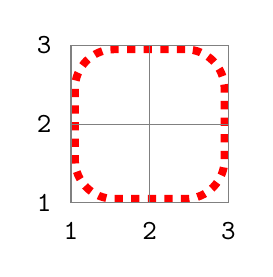
\begin{tikzpicture}

\draw (2.0, 2.0)
  node[draw, line width=0.1cm, dashed, color=red,
       rounded corners=0.5cm, inner sep=0cm] {

\begin{minipage}[t][1.9cm]{1.9cm}
\mbox{}

\end{minipage}

};\draw[gray] (1.0,1.0) -- (1.0,3);
\draw[gray] (2.0,1.0) -- (2.0,3);
\draw[gray] (3.0,1.0) -- (3.0,3);
\draw[gray] (1.0,1.0) -- (3,1.0);
\draw[gray] (1.0,2.0) -- (3,2.0);
\draw[gray] (1.0,3.0) -- (3,3.0);
\draw(1, 1) node [font=\ttfamily, label=below:{\texttt{1}}] {};
\draw(2, 1) node [font=\ttfamily, label=below:{\texttt{2}}] {};
\draw(3, 1) node [font=\ttfamily, label=below:{\texttt{3}}] {};
\draw(1, 1) node [font=\ttfamily, label=left:{\texttt{1}}] {};
\draw(1, 2) node [font=\ttfamily, label=left:{\texttt{2}}] {};
\draw(1, 3) node [font=\ttfamily, label=left:{\texttt{3}}] {};
\end{tikzpicture}

\end{center}

\end{document}
